\section{Consideraciones de diseño}

El diseño del prototipo se organiza como un ecosistema modular desacoplado para instrumentación, recopilación, procesamiento y análisis de manchas solares. Esta separación permite asignar responsabilidades claras a cada bloque: adquisición local junto al telescopio, preprocesamiento embebido, publicación de datos, inferencia mediante modelos de aprendizaje profundo, visualización web y análisis predictivo. La arquitectura busca que cada módulo pueda validarse y actualizarse de forma independiente, sin perder la trazabilidad entre imagen original, metadatos, recortes, clasificación Zurich--McIntosh y productos de tendencia temporal \citep{raspberryPi5Docs2026,zwoASI174Manual2025,luntWhiteLightWedges2026}.

\begin{figure*}[p]
    \centering
    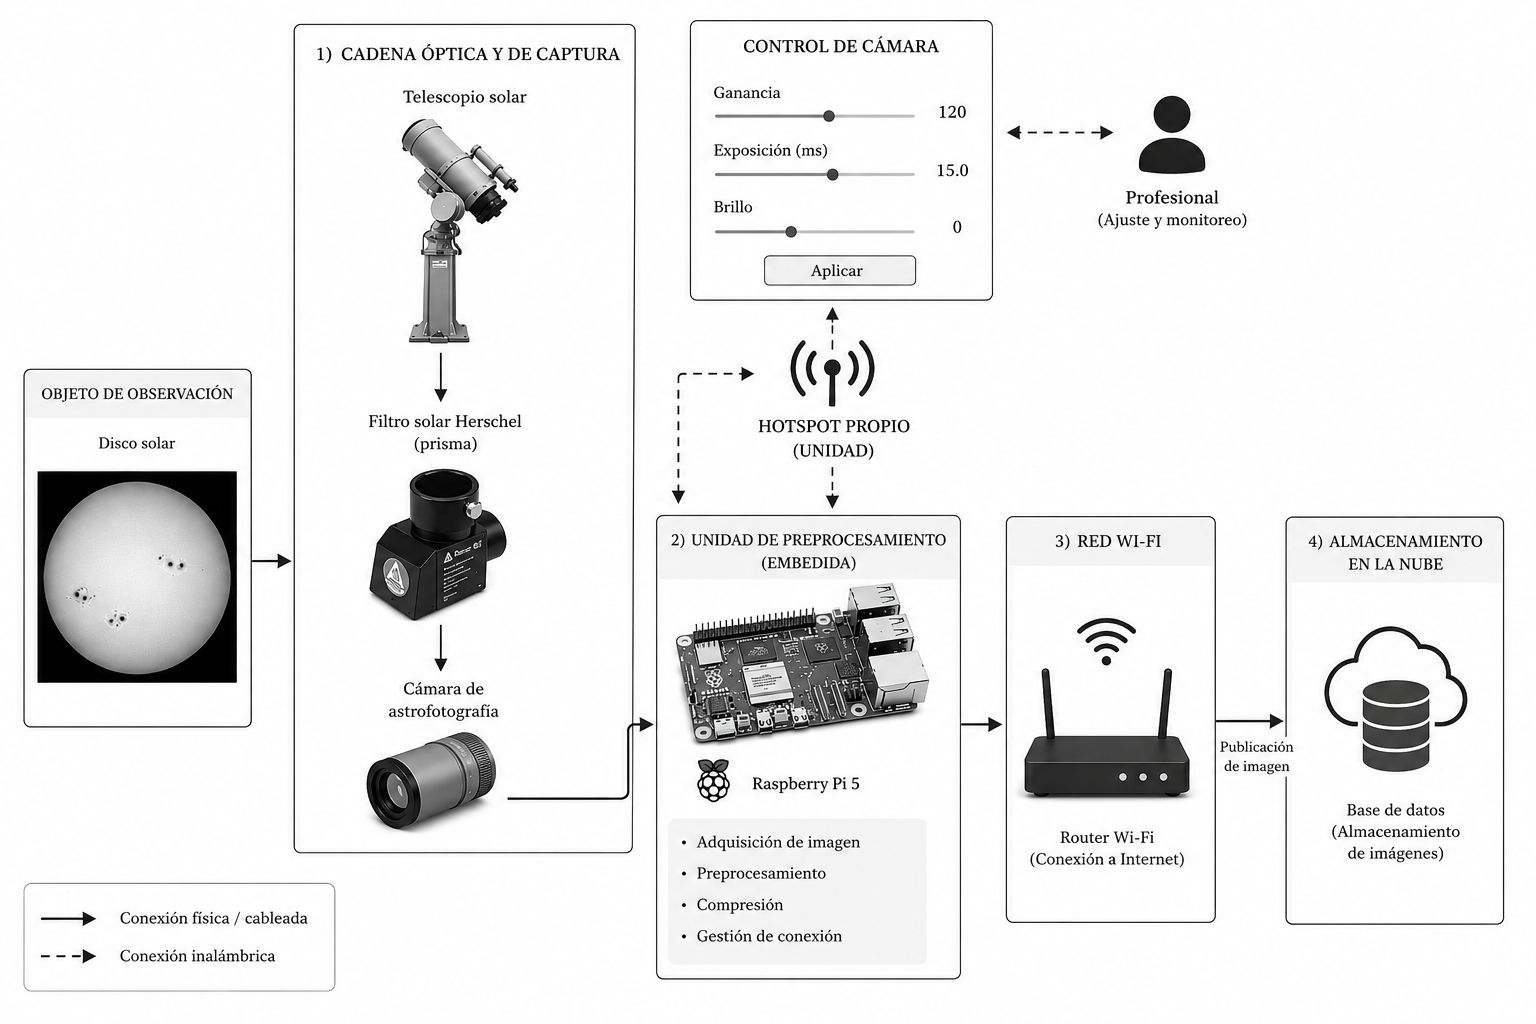
\includegraphics[height=0.38\textheight]{figures/hw/module.png}
    \caption{Flujo operativo de la etapa de preprocesamiento embebida. Se destacan la captura y calibración de imágenes de disco solar completo, la operación mediante panel web local y la publicación posterior hacia una base de datos en la nube. \textbf{Fuente:} Elaboración propia.}
    \label{fig:resumen-flujo-preprocesamiento-embebido}

    \vspace{0.25em}
    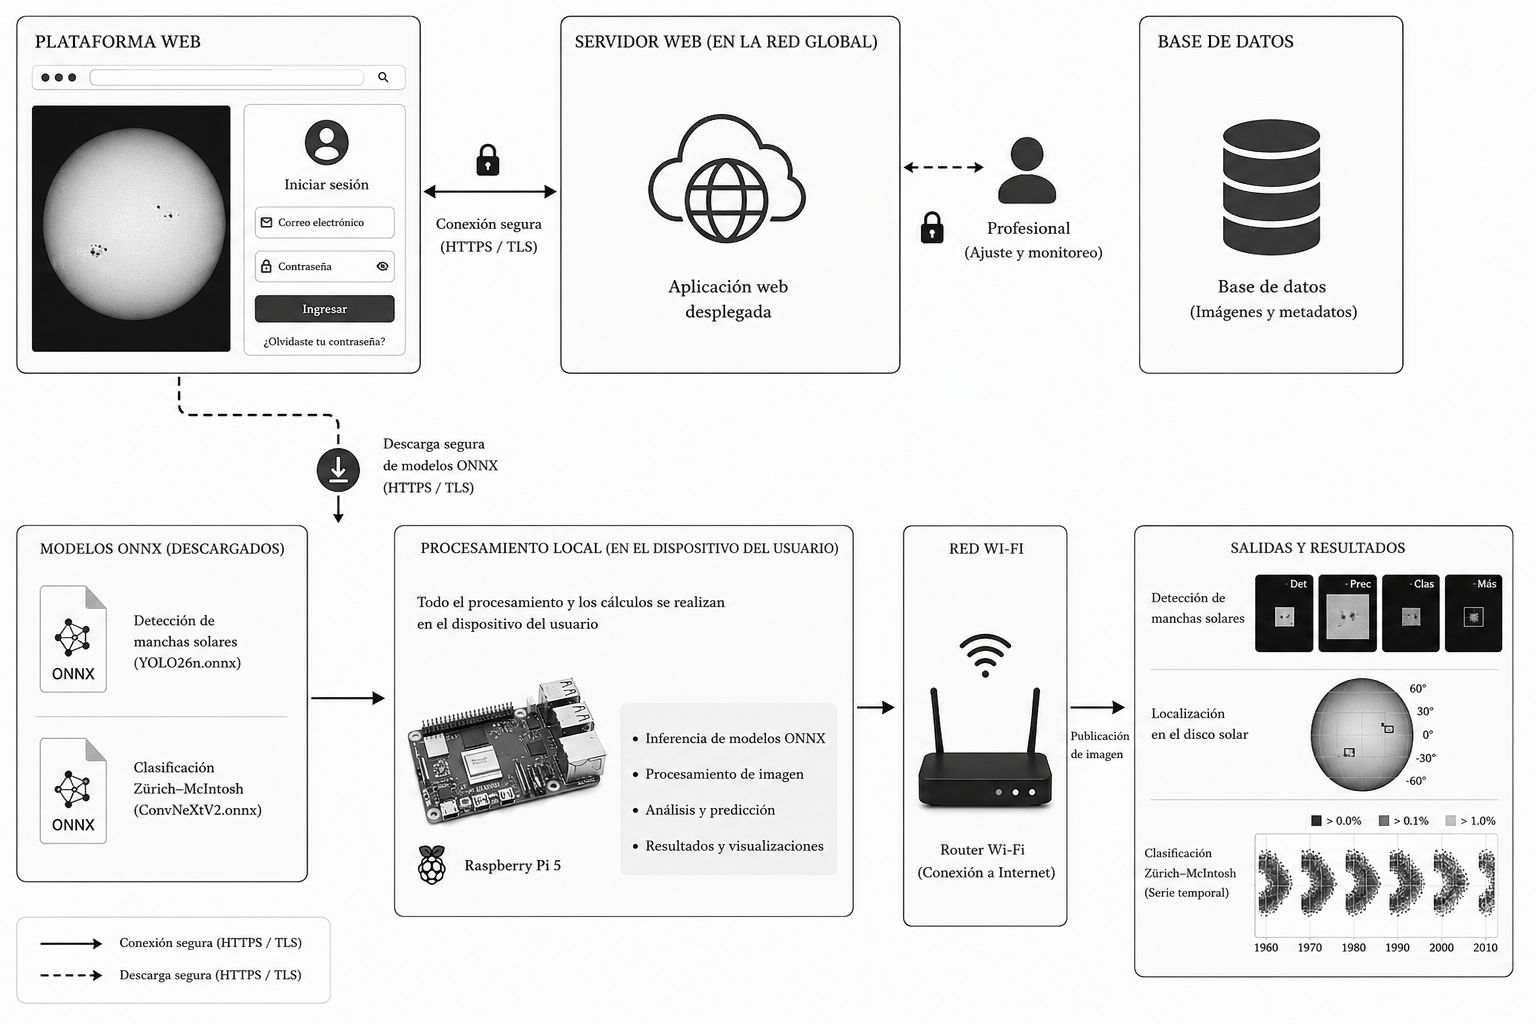
\includegraphics[height=0.38\textheight]{figures/hw/camera_mount.png}
    \caption{Flujo operativo de procesamiento, agrupamiento, clasificación ONNX y análisis predictivo de actividad solar. \textbf{Fuente:} Elaboración propia.}
    \label{fig:resumen-flujo-procesamiento-onnx}
\end{figure*}

Las Figuras~\ref{fig:resumen-flujo-preprocesamiento-embebido} y~\ref{fig:resumen-flujo-procesamiento-onnx} resumen las dos capas principales del flujo de trabajo. La primera corresponde a la unidad embebida que funciona junto al tren óptico y cumple una función dual de conectividad: puede generar una red WiFi local para configuración directa en campo o conectarse como cliente a una red disponible para sincronizar datos. Desde este nodo se controlan la calibración, la captura de imágenes de disco completo y los ajustes de exposición, ganancia y saturación. El panel web local evita depender de una estación externa permanente y permite supervisar el estado del dispositivo durante la observación.

La cámara seleccionada fue la ZWO ASI174MM Mini, principalmente por su sensor monocromático IMX174, obturador global, píxel de $5.86\,\mu\mathrm{m}$ y formato compacto. Estas características son relevantes para capturar estructuras fotosféricas con baja distorsión temporal y buen acoplamiento al tren óptico de observación solar \citep{zwoASI174Manual2025,sonyPregiusGlobalShutter,zwoGuideCameras2025}.

Una vez preprocesadas, las observaciones se publican en una base de datos que actúa como repositorio intermedio de imágenes, metadatos y registros observacionales. Esta decisión desacopla la captura de las etapas posteriores: la plataforma web puede consultar los datos disponibles, ejecutar modelos ONNX para agrupamiento y clasificación, presentar tendencias de actividad y conservar registros del Observatorio Astronómico ``Prof. Alexis Troche Boggino''. Así, el flujo no termina en la captura, sino que continúa hacia una capa abierta de análisis y consulta. La segunda capa integra la localización de grupos solares, la clasificación Zurich--McIntosh y la generación de contexto predictivo, manteniendo una cadena continua desde la instrumentación solar hasta la interpretación científica de los resultados.

\begin{figure*}[t]
    \centering
    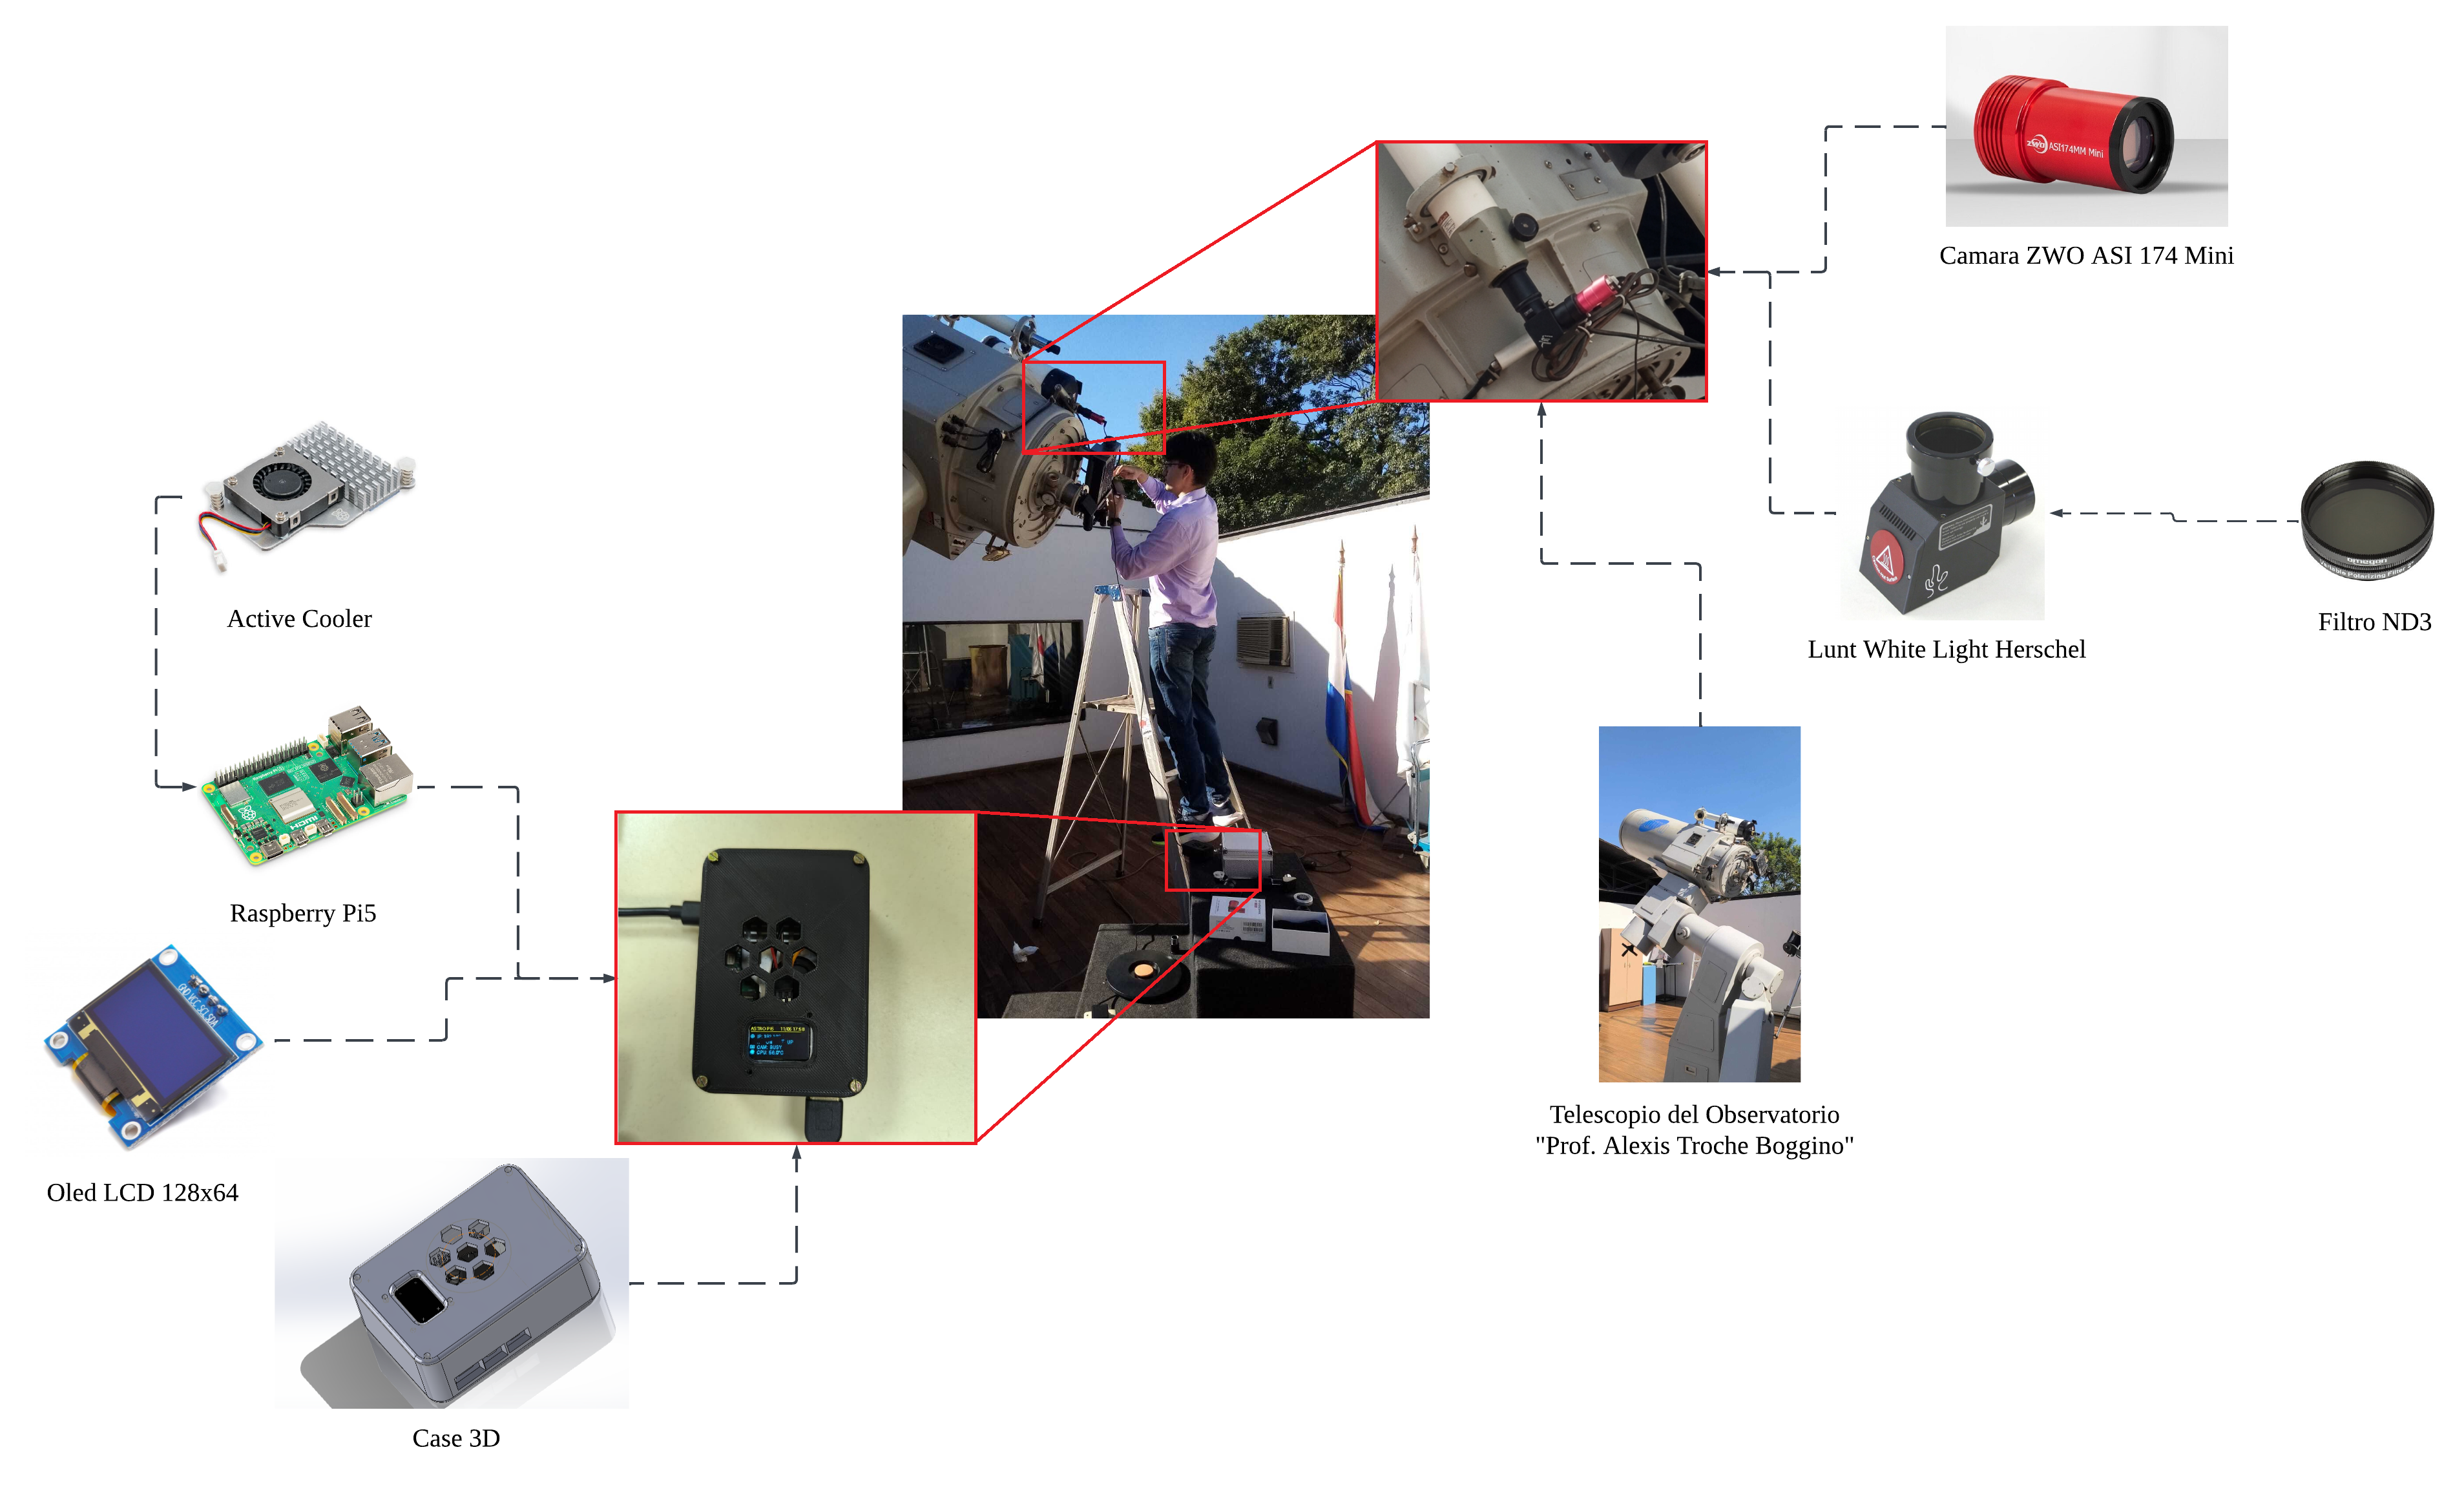
\includegraphics[width=0.9\linewidth]{figures/hw/hw_diagram.png}
    \caption{Componentes del flujo de adquisición de la imagen. \textbf{Fuente:} Elaboración propia.}
    \label{fig:resumen-componentes-adquisicion}
\end{figure*}

En cuanto a la cadena de procesamiento integrada en los modelos de aprendizaje profundo, se define como un modelo en cascada. Primero, el detector estima cajas $b_i=(x_i,y_i,w_i,h_i)$ para grupos solares; luego, cada recorte alimenta un clasificador jerárquico que estima probabilidades $p(Z\mid I)$, $p(P\mid Z,I)$ y $p(C\mid Z,P,I)$. La probabilidad conjunta se expresa como
\begin{equation}
    p(Z,P,C\mid I)=p(Z\mid I)\,p(P\mid Z,I)\,p(C\mid Z,P,I),
\end{equation}
lo que permite ordenar recomendaciones y descartar combinaciones no válidas \citep{mcintosh1990classification,woo2023convnextv2,cui2019classbalanced}.

Para el análisis predictivo se combinan dos representaciones: una escalar para el número de manchas solares y otra espacio-temporal para el diagrama de Spörer. En el modelo PVL--Kalman, la transición mensual se ajusta mediante un factor $\Phi_k$ y se corrige con la ganancia de Kalman $K_k$, mientras que DMD aproxima la evolución latitudinal mediante $\mathbf{x}_{k+1}\approx\mathbf{A}\mathbf{x}_k$ \citep{podladchikova2012kalman,kalman1960newapproach,schmid2010dmd,kutz2016dmd}.
